\begin{frame}
\frametitle{Transform feedback}
	\begin{itemize}
  \item Transform feedback stops rendering pipeline before rasterisation and sends primitives into buffers.
	\item It can be used in vertex shader and geometry shader.
  \item It can be combined with rendering (streams).
	\end{itemize}
	\begin{figure}[h]
	\includegraphics[width=10cm,keepaspectratio]{pics/tf_pipeline}
	\end{figure}
\end{frame}

\begin{frame}
\frametitle{Transform feedback}
	\begin{figure}[h]
	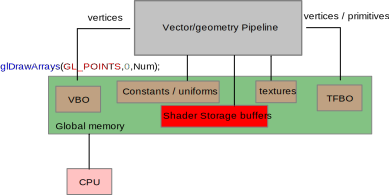
\includegraphics[width=10cm,keepaspectratio]{pics/tf_mem}
	\end{figure}
\end{frame}

\begin{frame}[fragile]
\frametitle{Transform feedback - example}
	{\scriptsize
	\begin{minted}[frame=lines]{c++}
const char*Vayrings[]={"Out1", "Out2"};
glTransformFeedbackVaryings(Program,2,Varyings,GL_SEPARATE_ATTRIBS);
glLinkProgram(Program);

//...

glBindBufferBase(GL_TRANSFORM_FEEDBACK_BUFFER,0,Buffer1);
glBindBufferBase(GL_TRANSFORM_FEEDBACK_BUFFER,1,Buffer2);

glEnable(GL_RASTERIZER_DISCARD);//nebudeme rasterizovat
//...
glBeginTransformFeedback(GL_TRIANGLES);
glDrawArrays(...);
glEndTransformFeedback();
	\end{minted}
	}
\end{frame}

\begin{frame}[fragile]
\frametitle{Transform Feedback - Inicialization}
  We have to link shader program with marked varyings.
	c++:
	{\scriptsize
	\begin{minted}[frame=lines]{cpp}
//list of variables that will be written into buffer(s).
const char*ResetVaryings[]={"vPosition","vVelocity","vMass"};
//set varyings and interleaving
glTransformFeedbackVaryings(ResetProgram,3,ResetVaryings,GL_INTERLEAVED_ATTRIBS);
//relink shader program
glLinkProgram(ResetProgram);
	\end{minted}
	}
	glsl:
	{\scriptsize
	\begin{minted}[frame=lines]{glsl}
#version 330

layout(location=0)out vec2  vPosition;//particle position
layout(location=1)out vec2  vVelocity;//particle velocity
layout(location=2)out float vMass;//particle mass
//...
void main(){
  vPosition = vec2(0);//init position
  vVelocity = vec2(cos(VelAngle),sin(VelAngle))*VelSize;//init velocity
  vMass     = Noise(MassSeed+uint(gl_VertexID),MinMass,MaxMass);//init mass
}
	\end{minted}
	}
\end{frame}

